\documentclass[12pt]{aghdpl}
% \documentclass[en,11pt]{aghdpl}  % praca w języku angielskim

% Lista wszystkich języków stanowiących języki pozycji bibliograficznych użytych w pracy.
% (Zgodnie z zasadami tworzenia bibliografii każda pozycja powinna zostać utworzona zgodnie z zasadami języka, w którym dana publikacja została napisana.)
\usepackage[english,polish]{babel}

% Użyj polskiego łamania wyrazów (zamiast domyślnego angielskiego).
\usepackage{polski}

\usepackage[utf8]{inputenc}

% dodatkowe pakiety

\usepackage{mathtools}
\usepackage{amsfonts}
\usepackage{amsmath}
\usepackage{amsthm}
\usepackage{array}
\usepackage{tabularx}

\newenvironment{conditions}
{\par\vspace{\abovedisplayskip}\noindent
\tabularx{\textwidth}{>{$}l<{$} @{${}={}$} >{\raggedright\arraybackslash}X}}
{\endtabularx\par\vspace{\belowdisplayskip}}


% --- < bibliografia > ---

\usepackage[
backend=biber,
style=numeric,
sorting=none,
%
% Zastosuj styl wpisu bibliograficznego właściwy językowi publikacji. 
language=autobib,
autolang=other,
% Zapisuj datę dostępu do strony WWW w formacie RRRR-MM-DD.
urldate=iso8601,
% Nie dodawaj numerów stron, na których występuje cytowanie.
backref=false,
% Podawaj ISBN.
isbn=true,
% Nie podawaj URL-i, o ile nie jest to konieczne.
url=false,
%
% Ustawienia związane z polskimi normami dla bibliografii.
maxbibnames=3,
]{biblatex}

\usepackage{csquotes}
% Ponieważ `csquotes` nie posiada polskiego stylu, można skorzystać z mocno zbliżonego stylu chorwackiego.
\DeclareQuoteAlias{croatian}{polish}

\addbibresource{bibliografia.bib}

% Nie wyświetlaj wybranych pól.
%\AtEveryBibitem{\clearfield{note}}


% ------------------------
% --- < listingi > ---

% Użyj czcionki kroju Courier.
\usepackage{courier}

\usepackage{listings}
\lstloadlanguages{TeX}

\lstset{
	literate={ą}{{\k{a}}}1
           {ć}{{\'c}}1
           {ę}{{\k{e}}}1
           {ó}{{\'o}}1
           {ń}{{\'n}}1
           {ł}{{\l{}}}1
           {ś}{{\'s}}1
           {ź}{{\'z}}1
           {ż}{{\.z}}1
           {Ą}{{\k{A}}}1
           {Ć}{{\'C}}1
           {Ę}{{\k{E}}}1
           {Ó}{{\'O}}1
           {Ń}{{\'N}}1
           {Ł}{{\L{}}}1
           {Ś}{{\'S}}1
           {Ź}{{\'Z}}1
           {Ż}{{\.Z}}1,
	basicstyle=\footnotesize\ttfamily,
}

% ------------------------

\AtBeginDocument{
	\renewcommand{\tablename}{Tabela}
	\renewcommand{\figurename}{Rys.}
}

% ------------------------
% --- < tabele > ---

\usepackage{array}
\usepackage{tabularx}
\usepackage{multirow}
\usepackage{booktabs}
\usepackage{makecell}
\usepackage[flushleft]{threeparttable}

% defines the X column to use m (\parbox[c]) instead of p (`parbox[t]`)
\newcolumntype{C}[1]{>{\hsize=#1\hsize\centering\arraybackslash}X}


\newenvironment{abstractpage}
{\cleardoublepage\vspace*{\fill}\thispagestyle{empty} }
{\vfill\cleardoublepage}
\renewenvironment{abstract}[1]
{\bigskip\selectlanguage{#1}%
	\begin{center}\bfseries\abstractname\end{center}}
{\par\bigskip}


%---------------------------------------------------------------------------

\author{Tomasz Kańka}
\shortauthor{T. Kańka}

%\titlePL{Przygotowanie bardzo długiej i pasjonującej pracy dyplomowej w~systemie~\LaTeX}
%\titleEN{Preparation of a very long and fascinating bachelor or master thesis in \LaTeX}

\titlePL{Sprzętowo-programowy system wizyjny do detekcji obiektów zwykorzystaniem termowizji}
\titleEN{Hardware-software vision system for object detection with the use of thermovision.}


\shorttitlePL{Sprzętowo-programowy system wizyjny do detekcji obiektów z wykorzystaniem termowizji} % skrócona wersja tytułu jeśli jest bardzo długi
\shorttitleEN{Hardware-software vision system for object detection with the use of thermovision.}

\thesistype{Praca dyplomowa magisterska}
%\thesistype{Master of Science Thesis}

\supervisor{dr inż. Tomasz Kryjak}
%\supervisor{Marcin Szpyrka PhD, DSc}

\degreeprogramme{Automatyka i Robotyka}
%\degreeprogramme{Computer Science}

\date{2018}

\department{Katedra Automatyki i Robotyki}
%\department{Department of Applied Computer Science}

\faculty{Wydział Elektrotechniki, Automatyki,\protect\\[-1mm] Informatyki i Inżynierii Biomedycznej}
%\faculty{Faculty of Electrical Engineering, Automatics, Computer Science and Biomedical Engineering}

%TODO uzupełnić lub usunąć
\acknowledgements{Serdecznie dziękuję \dots tu ciąg dalszych podziękowań np. dla promotora, żony, sąsiada itp.}


\setlength{\cftsecnumwidth}{10mm}

%---------------------------------------------------------------------------
\setcounter{secnumdepth}{4}

\begin{document}

\titlepages

\begin{abstractpage}
	\begin{abstract}{polish}

		
		\textbf{Słowa kluczowe:} 
		
	\end{abstract}
	
	\begin{abstract}{english}
	
		
		\textbf{Keywords:} 
		
	\end{abstract}
\end{abstractpage}

% Ponowne zdefiniowanie stylu `plain`, aby usunąć numer strony z pierwszej strony spisu treści i poszczególnych rozdziałów.
\fancypagestyle{plain}
{
	% Usuń nagłówek i stopkę
	\fancyhf{}
	% Usuń linie.
	\renewcommand{\headrulewidth}{0pt}
	\renewcommand{\footrulewidth}{0pt}
}

\setcounter{tocdepth}{2}
\tableofcontents
\clearpage

\chapter{Wstęp}
\label{cha:wstep}

Cyfrowa analiza obrazów znalazła szerokie zastosowanie w wielu dziedzinach życia. 
Umożliwia ona automatyczne uzyskanie istotnych dla rozważanego systemu informacji na podstawie obrazu bez konieczności angażowania człowieka.
%TODO jakiś przykład ?
Niektóre informacje zawarte w obrazie nie są dobrze dostrzegane przez ludzką percepcję np. kolor jest bardzo subiektywnym parametrem dla różnych ludzi. %TODO pomijając styl, to nie za bardzo rozumiem po co to zdanie - bardziej w nawiązaniu do Pana pracy byłoby pójście w kierunku kamer IR, termo, że percepcja u ludzi jest ograniczona itp.
Przez ostanie kilkadziesiąt lat opracowano tysiące różnych technik i algorytmów wyspecjalizowanych do określonych zadań np. kontrola jakości i przebiegu procesu przemysłowego, kontrola dostępu poprzez rozpoznawanie twarzy w smartfonach iPhone, optymalizacja ruchu na skrzyżowaniach, bezobsługowe systemy bezpieczeństwa i monitoringu, pojazdy autonomiczne, leśne fotopułapki do badania zachowań i migracji zwierząt itp. 
%TODO tu bym zastosował "gradację" od prostych do złożonych - a fotopułapka to chyba najprostsza jest.
Dzisiejsza technologia nie ogranicza nas tylko do stosowania spektrum światła widzialnego ludzkim okiem. 
Kamery na podczerwień stają się coraz tańsze i coraz bardziej popularne.
%TODO Proszę uważać, bo IR/na pod czerwień to co innego, a termowizyjne to co innego. Te pierwsze to wizyjne z zwiększoną czułością w paśnie podczerwonym. Ale może Pan o nich też wspomnieć.
Dostarczają nam informacje o temperaturze obserwowanych obiektów i jest coraz chętniej wykorzystywane w wielu różnych dziedzinach np. weterynarii do określenia miejsc urazów zwierząt, kontroli jakości artykułów spożywczych, analiza strat cieplnych w budynkach, detekcji gazów, systemów wspomagania kierowcy\cite{gade2014thermal}. 
%TODO dron, poszukiwania, policja, straż graniczna, gruzowsika..

Większość systemów wizyjnych służących do rozpoznawania przechodniów jest oparte o analizę obrazów z zakresu światła widzialnego, bądź podczerwieni. 
W przypadku światła widzialnego można uzyskać bardzo dobre wyniki pod warunkiem że wyszukiwane obiekty są dobrze oświetlone i wyróżniają się swoim kolorem od tła. 
Podczerwień, a szczególnie termowizja, umożliwia detekcję w warunkach nocnych i ograniczonej widoczności. %TODO tu też ostrożnie
Oba podejścia mają swoje wady i zalety, które wzajemnie się uzupełniają np. duże nasłonecznienia powoduje, że tło termiczne staje się dużo wyższe co utrudnia wyodrębnienie pieszego, natomiast daje idealne warunki do uzyskania dobrej jakości obrazu w zakresie widzialnym \cite{lee2015robust}. 
Połączenie tych dwóch obrazów daje możliwość uzyskania jeszcze lepszych metod rozpoznawania ludzi. %TODO nie metod, tylko skuteczności.
W pracy \cite{st2007combination} autorzy nazywają ten rozszerzony format jako RGBT (''Red-Green-Blue-Thermal''), natomiast inna praca jako analizę wielospektralną (Multispectral) \cite{hwang2015multispectral}, albo po prostu jako połączony obraz z kamery termowizyjnej i zwykłej\cite{lee2015robust}. 

Skuteczna detekcja obiektów jest często okupiona dużym zapotrzebowaniem na zasoby obliczeniowe. 
W wielu przypadkach nie da się uzyskać satysfakcjonującej wydajności by można było uznać system za działający w czasie rzeczywistym wykorzystując jedynie typowy komputer wyposażony w~procesor ogólnego przeznaczenia.
Daję to pole do popisu dla układów rekonfigurowalnych które mają możliwość dużego zrównolegnienia obliczeń. %TODO styl. "pole do popisu". Poza tym, by to bardziej ogólnie podszedł, że anceleracji i zahaczył o ASIC, GPU i FPGA, czy Zynq
Układy FPGA (ang. \textit{Field-Programmable Gate Array}) znalazły już zastosowanie w wielu systemach wizyjnych wykonując różnego rodzaju niskopoziomowe operacje kontekstowe, zamiany przestrzeni barw czy też binaryzacji nawet w czasie jednego cyklu zegara. 
%TODO No tu by się Pan bardziej postarał, bo to co Pan wymienił to początniem lat 90 robiono.
Dodatkową zaletą układów FPGA jest mały pobór mocy, co czyni je niezwykle atrakcyjne dla  aplikacji mobilnych -- takich jak drony czy czujniki środowiskowe \cite{garcia2014survey}. 

Niniejsza praca stanowi kontynuację i rozwinięcie pracy inżynierskiej autora.

\section{Cel pracy}


Celem pracy była realizacja wbudowanego systemu wizyjnego do detekcji wybranych obiektów (np. ludzi) na podstawie obrazu z kamery termowizyjnej. %TODO Tylko termo ?
Zakłada się, że jako platforma obliczeniowa zostanie użyty układ heterogeniczny (np. Zynq firmy Xilinx), który umożliwia realizację sprzętowo-programową algorytmów.

\section{Struktura pracy}

%TODO Tutaj standardowe "w rozdziele" + \ref{.}

W pierwszej części została opisana budowa cyfrowego systemu wizyjnego z wykorzystaniem połączonych obrazów RGB oraz IR. 
Zawiera on [rozdział] teorię stanowiącą podstawę dla realizowanych prac oraz kilka przykładów już zrealizowanych systemów. 
W następnym rozdziale została podana specyfikacja techniczna zastosowanych urządzeń oraz technologii. %TODO specyfikacja techniczna technologii dziwnie brzmi
W rozdziale czwartym opisano realizację autorskiego systemu detekcji ludzi. 
Prace zakończono omówieniem uzyskanych wyników, wnioskami oraz wskazaniem dalszych kierunków rozwoju stworzonego systemu.
\chapter{Cyfrowy system wizyjny}
\label{cha:csw}
%TODO mało inforamtywny tytuł.

%TODO Kilka zdań o zawratości rozdziału - szczególnie, że jest różnorodna.

%TODO Jak tam na to patrzę, to może być to podzielić dwa rozdziały:
%TODO podczerwień, kamery, kalibracja itp.
%TODO detekcja osób

\section{Podczerwień}

Mianem podczerwieni określa się promieniowanie elektromagnetyczne w zakresie fali o długości od 0,75 $\mu m$ do 1000~$\mu m$.
Każde ciało które ma temperaturę wyższą niż zero absolutne emituje swoją powierzchnią promieniowanie. 
Im większa jest temperatura ciała tym więcej promieniowania emituje. %TODO wyższa + powt. emituje
Dla każdej temperatury danego ciała istnieje charakterystyczna długość fali o najwyższej wartości mocy promieniowania. 
Wraz z wzrostem temperatury ta częstotliwość przesuwa się w zakres fal widzialnych. 
Można to zaobserwować, gdy stal osiąga wysoką temperaturę co skutkuję emisją światła. 

%TODO Tu by się przydało jakieś zdanie łączące, bo tak to się pojawia ni z gruchy...
Ciało doskonale czarne całkowicie pochłania padające na nie promieniowanie oraz emituję promieniowanie ściśle związane z jego temperaturą. 
Wykres na rysunku \ref{fig:perfect_black} przedstawia tą charakterystykę. 
Promieniowanie podczerwone jest częściowo pochłaniane przez atmosferę ziemską . 
Na rysunku \ref{fig:atmosfera_int} przedstawiono  tzw. transmisyjność atmosfery. 
W aparaturze rejestrującej w podczerwieni wykorzystuję się dwa zakresy przy których transmisyjność jest największa: 3 -- 5 $\mu m$ (MIWR, ang. \textit{mid wave infrared} -- podczerwień fal średnich) oraz 8 -- 14 $\mu m$ (LWIR , ang. \textit{long wave infrared} -- podczerwień fal długich)\cite{niklaus2007mems}.

\begin{figure}
\centering
\includegraphics[width=0.8\linewidth]{images/Atmosfaerisk_spredning}
\caption[Wykres transmisyjności atmosfery dla promieniowania podczerwonego ]{Wykres transmisyjności atmosfery dla promieniowania podczerwonego \cite{wiki:infrared}.}
\label{fig:perfect_black}
\end{figure}

\begin{figure}
\centering
\includegraphics[width=0.4\linewidth]{images/perfect_black_emi}
\caption[Emisyjność ciała idealnie czarnego]{Emisyjność ciała idealnie czarnego.}
\label{fig:atmosfera_int}
\end{figure}

%TODO Tu by się przydało coś o kamerach termowizyjnych napisać, albo nawet o kamerach wizyjnych i termowizyjnych, a dopiero potem o ich łączeniu.

\section{Metody akwizycji obrazu}
%TODO trzeba zmienić ten tytuł...

Większość implementacji wykorzystuje układ dwóch równoległych do siebie kamer, której przykład przedstawia rysunek \ref{dual_camera}.  %TODO tu trzeba napisać jawnie jakie to są kamery 
%TODO dlaczego od razu przejście do stereo
Często obrazy z kamer różnią się, wynika to z ich budowy, różnej rozdzielczości, kąta widzenia jak oraz zniekształceń soczewkowych.
Do poprawnego odwzorowania tej samej sceny w obu widmach należy zastosować algorytm mający na celu dopasowanie obu obrazów.
%TODO (tj. ..... /napisać co to jest dopasowanie/)

Pierwszym z etapów poprawnego dopasowania obrazów jest kalibracja.
Wykonuje się ją z~wykorzystaniem specjalnych plansz, które pozwalają określić położenie pewnych punktów w przestrzeni w obu rejestrowanych zakresach promieniowania. 
Punkty te pozwalają na obliczenie relacji między obrazami. 
Plansze mogą być aktywne (posiadają własne źródło ciepła) albo pasywne (przesłaniają obce źródło ciepła). 
W równoległym układzie kamer występuje również zjawisko paralaksy, które powiększa się wraz z wzrostem odległości obiektu od punktu kalibracji. 
W pracy \cite{hwang2015multispectral} autorzy zastosowali zwierciadło półprzezroczyste wykonane z wafla krzemowego pokrytego cynkiem do rozdzielenia obrazu w celu eliminacji tej wady (rysunek \ref{multispectral}).
%TODO Ten rysunek 2.3 b) jest jakiś nieczytelny i wymaga opisu/komentarza.

\begin{figure}[h]
\centering
\begin{subfigure}{0.45\textwidth}
\centering
\includegraphics[width=1\textwidth]{images/dual-camera}
\subcaption{\label{dual_camera}}
\end{subfigure}
\begin{subfigure}{0.45\textwidth}
\centering
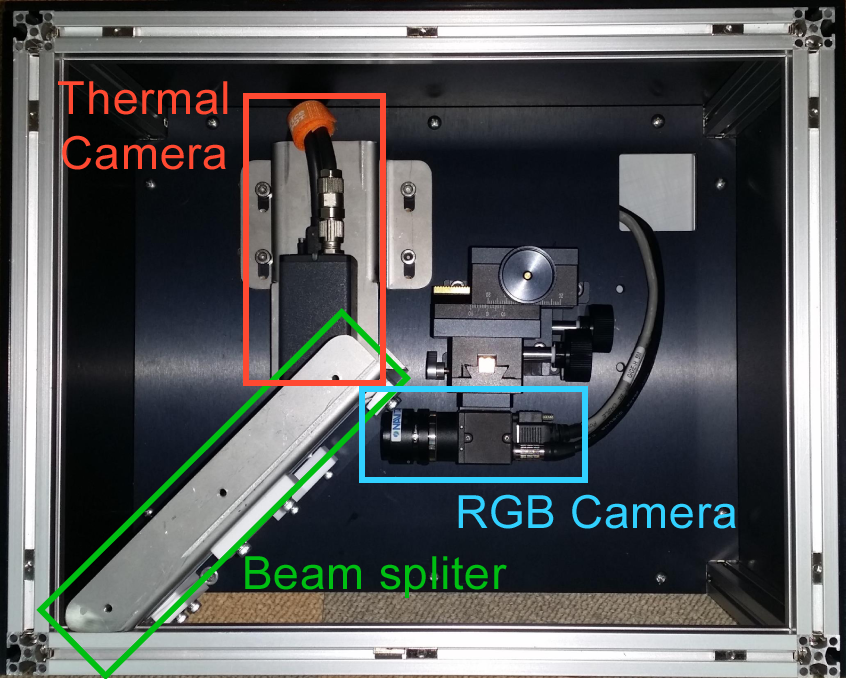
\includegraphics[width=1\textwidth]{images/multispectral}
\subcaption{\label{multispectral}}
\end{subfigure}
\caption{\label{fig:cameras_systems}Sposoby akwizycji obrazów: \protect\subref{dual_camera} dwie kamery równolegle \cite{lee2015robust}, \protect\subref{multispectral} z wykorzystaniem zwierciadła półprzezroczystego \cite{hwang2015multispectral}.}
\end{figure}


\section{Model geometryczny}
%TODO To chyba powinien być podrozdział - bo to jest wszczegółowienie tego ogólnego modelu integracji kamer.

Do opisu matematycznego systemu wykorzystuje się model kamery otworkowej. 
Dzięki niemu można opisać relację między trójwymiarową przestrzenią, a dwuwymiarowym obrazem za pomocą projekcji perspektywicznych. %TODO chyba perspektywicznej (projekcja jest jedna)
Nie stanowi on najdokładniejszego opisu matematycznego kamery, nie ma w nim uwzględnionych zakłóceń soczewkowych, dobre rezultaty w wielu aplikacjach.  %TODO czegoś brakuje np. jednakże  zapewnie dobre
Składa się ona z 2 zestawów parametrów: zewnętrznych oraz wewnętrznych.
%TODO Co to jest "ona" ale chyba trzeba już po prostu napisać Model, czy Transformacja
Parametry zewnętrzne definiują lokację kamery względem zewnętrznego układu współrzędnych. 
Są reprezentowane przez wektor translacji \(T\) między układem związanym z kamerą \( \left ( X_{c},Y_{c},Z_{c}\right ) \),
a zewnętrznym \(\left ( X,Y,Z\right )\). 
Drugim parametrem jest macierz rotacji \( R \) (między osiami tych dwóch układów).
Punkt \(P = \left [ X,Y,Z \right ]^T \) będący w zewnętrznym układzie współrzędnym ma swój odpowiednik w układzie wewnętrznym, który można określić zależnością 

\begin{equation}
P_{c} = RP+T
\end{equation}

Właściwości optyczne kamery można przedstawić w postaci macierzy kamery.
\begin{equation}
K = \begin{bmatrix}
f_x & 0 & x_0 \\ 
0 & f_y & y_0\\ 
0 &0 & 1
\end{bmatrix}
\end{equation}
gdzie:
\begin{conditions}
f_{x}, f_{y} & ogniskowa kamery wyrażona w liczbie pikseli, \\
x_{0},y_{0} & współrzędne punktu głównego. 
\end{conditions}

Macierz $K$ określa związek między znormalizowanymi współrzędnymi w układzie odniesienia kamery danych wzorem \(x_n = \frac{X_c}{Z_c}, y_n = \frac{Y_c}{Z_c}\), a~odpowiadającym im współrzędnymi punktów na obrazie \(u,v\):

\begin{equation}
\begin{bmatrix}
u \\
v \\
1
\end{bmatrix} = K \begin{bmatrix}
x_n \\
y_n \\
1
\end{bmatrix}
\end{equation}

%TODO To jest wszystko OK, ale nie ma tutaj wprost powiedziane jak dopasować dwa obrazy. Może jakiś przykład, ilustracja itp. Ogólnie omówienie jak wykonać taką kalibrację.


%TODO Osobny rozdział ....
\section{Algorytmy detekcji pieszych}

W cyfrowej analizie obrazu rozpoznawanie pieszych jest jedną z najbardziej aktywnie rozwijanych dziedzin. 
W przeciągu kilkudziesięciu lat powstało ponad tysiąc artykułów poruszających to zagadnienie \cite{zhang2015filtered}, w~których zaproponowano wiele różnych metod. 
Większość metod opiera się o analizę obrazu tylko w jednym spektrum: widzialnym albo podczerwieni. 
Praca \cite{hwang2015multispectral} pokazała że połączenie obu obrazów może dać lepsze wyniki. 
Podobnie w artykule \cite{gonzalez2016pedestrian} wykazano, że analiza multispektralna jest skuteczniejsza w dzień niż w nocy (o około 5\% AMR (ang. \textit{avrange miss rate}). 
W artykule \cite{benenson2014ten} autorzy podsumowują osiągnięcia w dziedzinie detekcji pieszych w latach 2004 -- 2014. 
Wyróżniono ponad 40 różnych podejść do problemu. 
Artykuł jest oparty o bazę danych Caltech-USA, która zawiera obrazy w~kolorze. %TODO Eksperymenty w artykule.... 
Jednym z wniosków jest, że przez ostanie dziesięć lat największy postęp został osiągnięty głównie dzięki dopracowaniu cech, które są wyodrębniane z obrazu niż ulepszanie klasyfikatora. 
Dodatkowo autorzy połączyli cechy dające najlepsze wyniki i stworzyli własną metodę która uzyska 12\% zysk AMR względem najlepszej badanej wcześniej metody.

%TODO a coś o głębokich sieciach ? Jakoś pominął Pan ten temat.

Dla typowego algorytmu detekcji pieszych można wyróżnić trzy podstawowe etapy:

\subsection{Ustalenie regionu zainteresowań} 

Jest to obszar zwany ROI (ang. \textit{region of interest}), w którym potencjalnie mogą znajdować się piesi. 
Wiele podejść uznaje cały obraz jako ROI i stosuje okno przesuwne sprawdzając każdy możliwy fragment obrazu. 
Jeżeli scena jest rejestrowana przez nieruchomą kamerę, ROI można określić poprzez różnicę między zapamiętanym tłem, a aktualnym obrazem (tzn. modelowanie i~odejmowanie tła). 
Wyodrębnienie ROI jest bardzo istotne w przypadku pracy w czasie rzeczywistym, ze względu na ograniczony czas analizy pojedynczego obrazu.

%TODO A jakieś inne metody wyodrębniania ROI

\subsection{Wyodrębnienie cech}

Do najbardziej popularnych cech można zaliczyć:

\begin{enumerate}
%TODO proszę to sprawdzić, bo zmieniłem gramatykę.
\item Histogramy zorientowanych gradientów (HOG). %TODO ang. skrót
Algorytm został zaproponowany przez N.Dalala i B. Triggs w pracy \cite{dalal2005histograms} i~stał się jednym z najbardziej popularnych technik w dziedzinie rozpoznawania ludzi. %TODO nie rozpozawania, tylko detekcji
Jest cały czas rozwijany i modyfikowany w wielu pracach naukowych.
Technika polega na zliczeniu kierunków gradientów, uzyskanych z 2 masek kierunkowych \(\begin{bmatrix}-1 & 0 & 1\end{bmatrix} \) i \( \begin{bmatrix}-1 & 0 & 1 \end{bmatrix}^T\), w komórkach o określonych wymiarach. 
Komórki te są organizowane w bloki, w obrębie których następuje normalizacja. 
Wektorem cech jest połączenie wszystkich histogramów z wszystkich bloków w jeden wektor.

%TODO Ciut więcej detali o tej metodzie (interpolacja, po co normalizacja itp.)

\item Lokalne wzorce binarne LBP (ang. \textit{Local Binary Paterns}).
Oryginalnie deskryptory te zaproponowane zostały do opisu tekstur. %TODO \cite też coś ojala 
Analizowany obraz zostaje podzielony na bloki. 
Następnie, do każdego piksela w bloku zostaje przypisany wzorzec binarny na podstawie wartości pikseli w jego sąsiedztwie. 
Jeżeli wartość sąsiadującego piksela jest większa od centralnego to przyjmuje on wartość 1. 
%TODO Tu coś dodac, że w ten sposobó...
Następnie zostaje obliczony histogram dla każdego bloku. 
Histogramy z wszystkich bloków wchodzących w skład obrazu tworzą wektor cech \cite{ojala2002multiresolution}.

\item Falki Haara.
Określają różnicę w kontraście między dwoma przylegającymi prostokątnymi obszarami. 
Są łatwe do skalowania i nie wymagają dużych nakładów obliczeniowych.

%TODO coś więcej

\item Kolor. W analizie obrazów wykorzystuje różne przestrzenie barw np. RGB, HSV oraz LUV.
%TODO też coś więcej. 

\item Lokalne struktury. W odróżnieniu od pojedynczych pikseli można wyznaczyć lokalne struktury o podobnym kolorze. (np. głowa i ręce mają podobne kolory, jednolita koszula, spodnie).
%TODO też coś więcej. Na jakiej zasadzie się ich używa.


\end{enumerate}

\subsection{Klasyfikator}
Otrzymany wektor cech jest poddany klasyfikacji, której wynik decyduje czy obraz zawiera człowieka.
W pracy \cite{benenson2014ten} autorzy wyróżnili 3 dominujące rodziny metod:

\begin{enumerate}
\item Rodzina DPM (ang. Deformable Part Detectors) ??? wykrywacze deformowlnych elementów ???. %TODO a nie Deformable Part Model ?
Technika polega na klasyfikacji poszczególnych elementów człowieka (głowa, tułów, nogi). Następnie jest analizowany układ tych elementów na obrazie i podjęcie decyzji o obecności człowieka.
%TODO ale ogólnie to prosze doczytać.

\item Deep networks – głębokie sieci neuronowe.

\item Decision forests – ?? lasy decyzyjne ?? zbiór nieskorelowanych drzew decyzyjnych.

\item inne: SVM (ang. support vector machine – maszyna wektorów nośnych), AdaBoost itp.


%TODO Też trzeba rozbudować ten opis. Poza tym te sieci głębokie to trzeba by omówić osobno.

\end{enumerate}

%TODO Nie omówił Pan specyfiki detekcji w podczerwieni.

%TODO Po tym ogólnym omówieniu oczekwiałbym bym jednak szegółowego omówienia publikacji. Najbardziej zależy mi na 4 z Poznania (nie wiem czy Panu podsyłąłem - mogę to zrobić.) Poza tym ma Pan tam kilka publikacji we wstepnie, o tej fuzji - może coś z tego. Opiać też metodę z inzynierki itp.




%TODO To chyba też osobny rodział. Powinien on zacząć się od omówienie technologii FPGA, Zynq i wykorzystywanej platformy sprzętowej.

\section{Wykorzystanie FPGA w analizie obrazu}

Tradycyjne systemy wizyjne zwykle bazują na architekturze sekwencyjnej.
W tym rozwiązaniu obraz jest sukcesywnie poddawany kolejnym przekształceniom, a~wyniki pośrednie zapisywane są w pamięci operacyjnej. 
W aplikacji procesorowej operacje te są wykonywane przez układ arytmetyczno-logiczny. 
Kolejne kroki algorytmu są kompilowane w ciąg instrukcji dla procesora ,który oprócz operacji matematycznych dużą część pracy poświęca na pobieranie i dekodowanie rozkazów oraz na odczytywanie i zapisywanie danych do pamięci. 
By taka aplikacja mogła pracować w czasie rzeczywistym, cała procedura musi wykonać się szybciej niż przychodzące dane obrazu, co wymusza wysokie taktowanie procesora sięgające kilku GHz. 
%TODO dodać, że to i tak nie zawsze pomaga. Poza tym wypada jakoś skomentować fakt istnienie procesorów wielordzeniowych.

W przypadku podejścia równoległego, implementacja poszczególnych kroków algorytmu odbywa się w osobnych procesach. 
Jeżeli kolejne kroki algorytmu wymagałyby danych otrzymanych z poprzednich, to zysk takiego zabiegu byłby równy zero. %TODO to jest dość niejednoznaczne. Musi Pan to opatrzyć jakimś lepszym komentarzem/przykładem.
By uzyskać znacznie przyspieszenie algorytm musi mieć możliwość podzielenia na wiele niezależnych części. 
Maksymalne do uzyskania przyspieszenie jest określone przez prawo Amdahla: 
\begin{equation}
P_w =\frac{1}{ s + \frac{1-s}{n_w}}
\end{equation}
gdzie:
\begin{conditions}
P_{w} & przyspieszenie algorytmu w systemie wieloprocesorowym, \\
s & cześć algorytmu niepodlegająca zrównolegleniu (wartość od zera do jeden), \\
n_{w} & liczba elementów obliczeniowych.
\end{conditions}

Teoretycznie jedynym ograniczaniem w możliwości zrównoleglenia obliczeń jest liczba zasobów dostępnych, jednak istotnym aspektem jest sposób dostarczania danych do zaimplementowanych w układzie procesorów. %TODO procesorów, czy modułów obliczeniowych - no bo w sumie to musi się Pan ogólnie zdecydować, czy pisze to Pan ogólnie, czy z uzględnieniem architektury.
Czas i przepustowość jaka jest potrzebna do odczytania i zapisu obrazu po przetworzeniu z i do pamięci jest najczęściej wąskim gardłem systemu wizyjnego. %TODO to z i do źle wygląda
Z tego powodu przetwarzanie obrazu bezpośrednio z sensora w czasie jego akwizycji jest chętnie wykorzystywane, gdyż zmniejsza to liczbę operacji odczytu i zapisu. \cite{garcia2014survey}

%TODO No i w ten sposób to Pan w rodziale o FPGA, ani razu nie użył słowa FPGA.
%TODO Druga sprawa to jest GPU - tez się tu powinno pojawić.


%TODO To trzeba wkomponować w rozdział o algorytmach. Ew. rozdział FPGA można dać przed algorytmy i wtedy omówić metody programowe oraz sprzętowe.
\section{Przegląd literatury}

\subsection{Podobne rozwiązania}
%TODO ponieważ te opisy są dość obszerne proszę jednak dać to w osobne podrozdziały subsub (czy jak to wyjdzie)

W pracy \cite{kolzpoz} autorzy opracowali algorytm pozwalający na szybką i efektywną detekcję przechodniów w czasie rzeczywistym. 
Termowizja pozwala na uzyskanie dobrego kontrastu między poszukiwanym przechodniem a otoczeniem. 
System dedykowany jest do pracy w nocy, kiedy kontrast między człowiekiem pozwala na jednoznaczne ich rozróżnienie.  %TODO między człowiekiem, a czym ?
Rozwiązanie bazuje na ulepszonym algorytmie progowania i segmentacji obrazu. 

Pierwszym etapem jest wyodrębnienie obszarów zainteresowań (ROI). 
Pozwala to na znaczne ograniczenie obszaru obrazu do analizy. %TODO rozmiaru analizowanych fragmentów obrazu (czy jakoś tak)
Obraz w odcieniach szarości zostaję poddany binaryzacji z użyciem dwóch progów: mniejszym i większym. 
Dodatkowo każdy wykryty obszar tworzy dodatkowy ROI przylegający do pierwotnego. %TODO 1. powt. dod, 2. niejasen
Progowanie z pojedynczym progiem jest niewystarczające w wielu wypadach dlatego autorzy zastosowali podwójne progowanie. %TODO ale to już Pan napisał wcześniej.
Pozwala to na detekcję przechodniów w różnych rejonach obrazu o różnym kontraście. 
Progi zmieniają się wraz z dynamiką obrazu wejściowego. 
%TODO Proszę to kwestię dwóch progów lepiej opisać. Bo nie wiadomo jak co i po co jest robione.
W obrazie termicznym człowieka często występuję obszar o niższej temperaturze w okolicach bioder. 
Skutkuje to przerwą w zbinaryzowanym obiekcie i błędną klasyfikację np.: samych nóg. 
Autorzy opracowali technikę polegającą na powiększeniu obszaru. 
Łączy ona dwie połówki człowieka, jeżeli posiadają one wspólne współrzędne wzdłuż pionowej osi tworząc nowy obszar. %TODO to "tworząc" coś nie pasuje
Ostatecznie obie grupy obszarów zainteresowania uzyskanych z obu progowań zostają połączone. %TODO to też jest niejasne. 

Następnym krokiem jest filtracja wyników. 
Ma ona na celu zredukowanie liczby obszarów przed końcową analizą. 
Autorzy zastosowali filtrację opierającą się na proporcji obszaru zainteresowań. 
Pozytywnie zakwalifikowane zostały tylko obszary o odpowiednich proporcja wysokości do szerokości (1:1.3 do 1:4). 
Z racji, że badany obraz pochodzi z kamery zamontowanej na stałe na samochodzie, autorzy wykorzystali filtrację perspektywiczną. 
W większej odległości na horyzoncie obiekty są mniejsze. %TODO tu jest coś nie tak...
Zakłada ona że w określonych obszarach obrazu istnieje maksymalna możliwa wysokość kandydata. 
Filtracja jednorodnych regionów pozwoliła na odrzucenie obszarów, które często występują jako część szerszych obiektów nie mających nic wspólnego z przechodnimi. %TODO To jest niejasne...
Autorzy zaproponowali obliczenie odchylenia standardowego tych obszarów w odcieniach szarości i odrzucenie części, która jest poniżej pewnego progu. 

Ostatnim krokiem algorytmu jest klasyfikacja wytypowanych kandydatów. 
Autorzy wykorzystują histogram zorientowanych gradientów jako deskryptor tworząc wektor 3780 cech, które są następnie klasyfikowane przez SVM.

W celu zbadania dokładności algorytmu został przeprowadzony test na zbiorze CVC-14, który zawiera obrazy nagrane kamerą FIR podczas nocnego przejazdu samochodem. 
Testy wykazały, że metoda podwójnego progowania daje trzy razy lepsze rezultaty, niż przy wykorzystaniu pojedynczego progu. 
Wraz z zaproponowanymi technikami filtracji zaowocowało to bardzo efektywnym mechanizmem segmentacji. %TODO no właśnie segmentacji czy klasyfikacji
Cała procedura detekcji przechodniów osiągnęła wysoki poziom wydajności na poziomie 33 klatek na sekundę przy wykorzystaniu pojedynczego rdzenia CPU.
%TODO A dla jakich parametrów strumienia wizyjnego.


W pracy \cite{suard2006pedestrian} autorzy zaproponowali wykorzystanie dwóch kamer termowizyjnych tworząc system stereowizyjny. 
By wyodrębnić obszary zainteresowania, w~których potencjalnie znajdują się przechodnie, zgrupowano piksele o wartościach powyżej kilku różnych progów.
%TODO znowu za mało szczegółów...
Porównując te dwa obrazy można określić pozycję i odległość źródła ciepła od kamery. 
W obrazie termowizyjnym człowieka można zauważyć, że najbardziej ciepłym i odsłoniętym obszarem ciała jest głowa. %TODO to raczej, z tego że ZWYKLE głowa (stricte twarz) ew. dłonie sa odsłoniete, wynika, że sa widoczne jako najcieplejsze... bo tak ogólnie to chyba temperatura jest względnie równomiarna.
Wykorzystując ten fakt oraz informację o odległości od kamery, zostają wytyczone obszary wokół tych pikseli o wielkości zależnej od tej odległości.
%TODO No to jest kompletnie niejasne...
Następnie wszystkie wyodrębnione tak obszary zostają przeskalowane do wymiaru 128x64 piksele i poddane klasyfikacji za pomącą kombinacji HOG+SVM. 
W tej pracy autorzy skupili się na optymalnym doborze parametrów deskryptora HOG. 
Badania zostały przeprowadzone na bazie obrazów termowizyjnych o wymiarach 128x64. 
Zestaw zawierał 4400 obrazów: 2200 próbek z pieszymi oraz 2200 bez pieszych. 
Został wykorzystany następujący zestaw parametrów HOG:
\begin{enumerate}
\item wielkość komórki: 4x4, 8x8, 16x16,
\item wielkość bloku: 1x1, 2x2, 4x4,
\item nakładanie się bloków: 1, 2, %TODO to nie wiadomo co oznacza
\item liczba przedziałów histogramu: 4, 8, 16, %TODO jw. (szzcególnie, że std. jest 9)
\item metoda dopasowania: ważony lub nie %TODO kompletnie nie wiadomo
\item metoda normalizacja bloku: L1, L2, brak %TODO to ew. będzie wiadomo, jak to wcześniej opisze.
\end{enumerate}

Parametry dla klasyfikatora SVM :
\begin{enumerate}
\item wielkość zestawu do nauki: 10, 100, 1000 obiektów na klasę,
\item waga źle sklasyfikowanych punktów C: 0.01, 1, 100.
\end{enumerate}
%TODO Wnioskuję, że to liniowy SVM był - proszę to jawnie napisać.
Autorzy przeprowadzili po 10 procedur uczenia klasyfikatora dla każdej kombinacji wykorzystując różne kombinacje danych do nauki i testów. 
Po przeprowadzonych badaniach został wytypowany optymalny zestaw parametrów:
\begin{enumerate}
\item Wielkość komórki: 8x8, 
\item wielkość bloku: 2x2
\item nakładanie się bloków: 1,
\item liczba przedziałów histogramu: 8
\item metoda dopasowania histogramu: ważona 
\item metoda normalizacja bloku: L2.
\end{enumerate}
Badanie parametrów dla klasyfikacji SVM wykazało, że im większy zestaw uczący tym lepszą można uzyskać skuteczność detekcji. 
Parametr C miał marginalne znaczenie na końcową skuteczność.


%TODO Opis tego trzeciego algorytmu jest to poprawki !!!

Autorzy pracy \cite{nanda_2002} przedstawili metodę opartą o wzorzec probabilistyczny i klasyfikator Bayesa. 
Obraz wejściowy zostaje zbinaryzowany z zadanym progiem. 
Próg ten nie jest stały i zależy od wielu czynników. %TODO a można konkretniej ? Np., że zostało to omóione poniżej
Autorzy bazując na danych uczących stanowiących 1000 prostokątnych okien o rozmiarze 48x128 pikseli zawierających przechodnia średnią oraz odchylenie standardowe wartości dla pikseli należących do obrazu przechodnia \( \mu_1 \sigma_1 \) bądź tła \( \mu_2 \sigma_2 \) a następnie obliczyli próg binaryzacji za pomocą równia \ref{eq:treshold_nanda}. %TODO odwołania do równiań poprzez eqref. , te symbole jakoś w tekście nie są w nawiasie
%TODO To zadnie to jest jakiś "potworek" proszę poprawić.

\begin{equation} \label{eq:treshold_nanda}
threshold = \frac{\sigma_1 \sigma_2}{ \sigma_1 + \sigma_2} \ln\left ( \frac{\sigma_1}{\sigma_2} \right ) + \frac{\sigma_1\mu_1 + \sigma_2\mu_1}{\sigma_1+\sigma_2}\end{equation}

Aby uzyskać wzorzec prawdopodobieństwa, zbiór testowy został zbinaryzowany z uprzednio wyliczonym progiem. 
Następnie zostało obliczone prawdopodobieństwo przynależności piksela do przechodnia we wzorcu. %TODO To jest ciut niejasne.
Mając już wzorzec, został obliczony combinedpropability ze wzoru \eqref{eq:combo_nanda} dla 1000 okien zawierających i nie zawierających człowieka oraz wyciągnięta średnia i odchylenie standardowe dla nich. %TODO To com.... to trzeba na coś zamienić !!!
Dało to podstawę do obliczenia progu dla wartości combinedpropability z wzoru \eqref{eq:treshold_nanda}. 
%TODO to jest jakieś niejasne.

\begin{equation} \label{eq:combo_nanda} combinedprobability(i,j)=\sum_{x=1}^{48}\sum_{y=1}^{128}(th(x,y)*p(x,y)+(1-th(x,y))*(1-p(x,y)))\end{equation}
\noindent
gdzie \(th(x,y)\) to okno wokół piksela \((i,j)\), a \(p(x,y)\) to wzorzec prawdopodobieństwa wystąpienia pieszego.

Badana klatka obrazu jest badana poprzez okno przesuwne tworząc mapę prawdopodobieństwa. %TODO badana klatka jest badana ? 
Wartości które przekroczą próg wskazują, że w danym oknie znajduje się człowiek. %TODO ale jakie wartości ? 
Autorzy zbadali algorytm na 6 sekwencjach filmowych i uzyskali wynik między 75\%-90\% wykrycia przy jednym fałszywym wykryciu na ramkę. %TODO chyba średnio jednym...


%TODO Tutaj omówienie tych algorytmów z Poznania

\subsection{Podejście sprzętowo - programowe}

W pracy \cite{honegger2014real} autorzy wykorzystali układ FPGA oraz CPU małej mocy do skonstruowania systemu wizyjnego dla robotów. 
System analizował obraz steroskopowy z dwóch kamer tworząc mapę głębi. %TODO wizyjnych, czy termo
Obie kamery są bezpośrednio podpięte do układu FPGA, w którym obrazy są przetwarzane. %TODO proszę zwrócić uwagę na czas -> były (bo wcześniej wykorzystali) ogólnie takie badania opisuje się w czasie przeszłym.
Następnie dwa oryginalne obrazy oraz mapa głębi są przesyłane do CPU za pomocą specjalnej szyny danych. %TODO może magistrali
Moduł \textit{frame grabbera} przechwytywał ten obraz i wykorzystując DMA (ang. \textit{Direct Memeory Acces}) zapisywał do pamięci systemu. 
Ten zabieg gwarantował poprawną transmisję obrazu do CPU. 
Rozdzielczość oraz liczba klatek na sekundę są w pełni elastyczne, dzięki czemu CPU dostawało obraz o szerokości trzy raz większej niż oryginalny obraz.
%TODO no to jest niejasne... tzn. ta pierwsza część zdania.
Pozwalało to na przesłanie zsynchronizowanego lewego, prawego obrazu i mapy głębi. 
System pracował w rozdzielczości 752x480 piksle i 60 klatkach na sekundę. 
Całość, włącznie z kamerami, układem FPGA, CPU oraz konwerterami napięcia pobierał mniej niż 5W mocy. 
Całkowita latencja podana przez autorów rozwiązania wynosi około 2ms.

%TODO ale to coś jeszcze robiło ? Bo rozumiem, że FPGA liczyło stereo (pytanie jak) i do CPU trafiały te obrazy. Ale coś więcej się działo ?

W pracy \cite{piao2016real} autorzy wykorzystali układ SoC (ang. System on Chip) do detekcji pieszych dla zaawansowanego systemu wspomagania kierowcy (ADAS ang. \textit{advanced driver assistance system}). 
Głównym wyzwaniem było opracowanie metody, która działa w czasie rzeczywistym, ma mały pobór mocy oraz niski koszt wykonania. %TODO raczej systemu/rozwiązania (szczególnie koszt wykonania dla algorytmu jest dyskusyjny)
Większość topowych algorytmów wymaga znacznych zasobów obliczeniowych. %TODO topowych -> słowo potoczne i do zmiany
Autorzy dokonali zatem relaksacji problemu poprzez zastosowanie prostszego deskryptora jakim jest LBP oraz klasyfikatora SVM. 
Autorzy zamontowali po każdej stronie pojazdu inteligentną kamerę o 180$^\circ$ horyzontalnym kącie widzenia by jak najlepiej monitorować przestrzeń wokół niego. %TODO wyeliminiować powt. autorzy
W kamerach została przeprowadzona wstępna obróbka obrazu (rektyfikacja i skalowanie). %TODO rektyfikacja ? czyli to był system stetero ?
Przetworzony obraz z kamer był transmitowany do ,,Fusion-Box'', gdzie odbywała się generacja kandydatów, klasyfikacja, weryfikacja oraz śledzenie. 
Wyniki były przesyłane do wbudowanego komputera PC. 
Rozwiązanie nie zostało jeszcze w pełni zaimplementowane, ale pierwsze testy dawały obiecujące rezultaty.

W pracy \cite{xiao_2015} autorzy wykorzystali układ FPGA i naiwny klasyfikator Bayesa do detekcji przechodniów w obrazie termowizyjnym. 
Klasyfikator zakłada, że wszystkie predykatory są niezależne od siebie. 
Szanse na wystąpienie przechodnia w oknie są 50/50 (jest albo nie ma), problem sprowadza się do za pomocą równania: %TODO do za ??? poza tym to jest coś niejasne}

\begin{equation} \label{eq:bayes_china}
\sum_i \ln p(w_i|P) > \sum_i \ln p(w_i|\bar{P})
\end{equation}

\noindent gdzie \( p(w_i|P) \) to prawdopodobieństwo że piksel $w_i$ przynależy do obrazu człowieka
\( p(w_i|\bar{P}) \) przynależy do tła.
%TODO no ale co to jest i, bo czegoś tu nie rozumiem....

Jeżeli wyrażenie jest prawdziwe, to w badanym oknie znajduje się człowiek. 
Autorzy na podstawie 60 pozytywnych próbek utworzyli macierz rozkładu prawdopodobieństwa PDM (ang. \textit{probability distribution matrix}). 
W celu usprawnienia obliczeń w układzie FPGA przeskalowali prawdopodobieństwo na wartości całkowitoliczbowe w zakresie od 1 do 127. 
Następnie obliczono logarytm o podstawie dwa z uzyskanej macierzy i jej odwrotności (poprzez odjęcie od 128 wartości macierzy pozytywnej), a następnie pomnożono przez 32. %TODO powt. następne
Utworzono tak dwie macierze: LPDW i LPDB dla białych i czarnych pikseli. (ang. \textit{logarithmic probability matrix} – logarytmiczna macierz prawdopodobieństwa). 
Przyjęto, że prawdopodobieństwo przynależności piksela do tła jest stałe i wynosi 50\%, co daje wartość 192 po uprzednich przekształceniach. 
Ostatecznie obecność człowieka w oknie oblicza się z wzoru: %TODO raczej klasyfikacji dokonuje się...

\begin{equation}\label{equ:Lp}
L_{p} = \sum_{x=1}^{j}\sum_{y=1}^{k}(th(x,y)*LPMW(x,y)+(1-th(x,y))*LPMB(x,y))
\end{equation}
\begin{equation}\label{equ:Lb}
L_{b} = j*k*192
\end{equation}
\begin{equation} \label{equ:ispedistant}
IsPedestrian = \left\{ \begin{array}{ll}
1 & \textrm{gdy $L_{p} \geq L_{b} + K$}\\
0 & \textrm{gdy $L_{p}<L_{b} + K$}
\end{array} \right.
\end{equation}

\noindent gdzie $j$ i $k$ stanowią wysokość i szerokość okna przesuwnego. Wartości $L_p$ i $L_b$ odnoszą się do sum prawdopodobieństw przynależności białego/czarnego piksela do obrazu człowieka. W praktyce, każdy piksel w oknie może przyjąć jedną z dwóch wartości, co odwzorowuje jak mocno jest dopasowany do wzorca. %TODO styl. odwozorowuje do wzorca.

%TODO ogólnie ta metoda (z p. inż. też jest jakoś nie do końca fajnie opisana) - proszę to dopracować.
%TODO dalej - proszę "pochwalić" się artykułem na ten temat - przecież powstał





\chapter{Wykorzystane zasoby sprzętowe i technologie}
\label{cha:hw}
\section{Kamera termowizyjna Lepton}

\begin{figure}[h]
    \centering
    \includegraphics[width=0.6\textwidth]{images/Lepton}
    \caption{Widok poglądowy na kamere Flir Lepton.}
    \label{fig:lepton}
\end{figure}
 
Lepton jest zintegrowaną w pojedynczym układzie kamerą składającą się z soczewki, sensora podczerwieni fal długich (ang. LWIR – long wave infrared) oraz elektroniki sterującej i przetwarzającej sygnał. Checuje siębardzo małymi wymiarami co czyni go idealnym do zastosowań mobilnych. Układ ma możliwość domontowania dodatkowej przesłony która jest wykorzystywana do automatycznej optymalizacji procesu ujednolicania obrazu (kalibracji sensora).
Prosty do integracji z dowolnym mikrokontrolerem dzięki zastosowaniu standardowych protokołów i interfejsów. Lepton po podłączeniu od razu pracuję w domyślnym trybie pracy, który może zostać zmieniony za pomocą CCI (ang. camera control interface – interfejs kontroli kamery).\cite{lepton}
Parametry:
\begin{itemize}
\item Wymiary: 11,8 x 12,7 x 7,2 mm, 
\item Sensor: niechłodzony mikrobolometr VOx (tlenek wanadu),
\item Rejestrowany zakres: fale długie podczerwieni, 8$\mu m$ do 14$\mu m$ ,
\item Wielkość piksela: 17 $\mu$m,
\item Rozdzielczosć: 80x60 pikseli,
\item Ilość klatek na sekundę 8,6,
\item Zakres rejestrowanych temperatur: -10  $^\circ$  C 140  $^\circ$  C (Tryb wysokiego wzmocnienie),
\item korekta niejednorodności matrycy: automatyczna na bazie przepływu optycznego
\item kąt widzenia horyzontalny / diagonalny: 51 $^\circ$ \\ 66 $^\circ$,
\item Głębia ostrości: od 10cm do nieskończoności
\item Format wyjściowy: do wyboru: 14-bit, 8-bit (z AGC (ang. automatic gain control – automatyczna kontrola wzocnienia)) 24-bit rgb (z ACG i koloryzacją).
\item Interfejs video: VoSPI (Video over Serial Peripherial Interface)
\item Interfejs sterujący: CCI (I2C podobny)
\end{itemize}
\section{Zynq-7000}

Rodzina układów Zynq-7000 bazuje na architekturze SoC (ang. System on Chip). Posiadają zintegrowany kompletny system składający podzielonego na dwie części: systemu procesorowego bazującego na procesorze ARM Cortex-A9 (PS ang. Porcessing System) oraz logikę programowalną (PL ang. programable logic) FPGA w jednym układzie scalonym. Na rysunku \ref{fig:zynq7000} przedstawiono schemat architektury. Prócz procesora cześć procesorowa posiada wbudowaną pamięć, kontroler pamięci zewnętrzne oraz szereg interfejsów dla układów peryferyjnych takich jak USB, GigEthernet, CAN, I2C, SPI. W części logiki programowalnej znajdują się bloki logiki konfigurowalnej (CLB ang. configurable logic block), 36Kb bloki pamięci RAM, procesory sygnałowe DSP48, układ JTAG, układy zarządzania zegarami oraz dwa 12-bitowe przetwornik analogowo-cyfrowy.

Komunikacji między częścią procesorową a logiką programowalną odbywa się za pośrednictwem Interfejsu AXI (ang. Advanced Extensible Interface), oraz bezpośrednio wykorzystując porty generalnego przeznaczenia, przerwania, oraz poprzez bezpośredni dostęp do pamięci (DMA ang. Direct Memory Access) 

\begin{figure}[h]
    \centering
    \includegraphics[width=1\textwidth]{images/Zynq-7000-Overview}
    \caption{Schemat ogólny architektury układu Zynq-7000.}
    \label{fig:zynq7000}
\end{figure}

\section{Interfejs AXI}
 AXI (ang. Advanced eXtensible Interface zawansowany rozszerzalny interfejs) jest częścią ARM AMBA (ang. Advanced Microcontroller Bus Architecture) – otwartego standardu, specyfikacją do zarządzania i połączeń między blokami funkcyjnymi w SoC. Aktualnie jest stosowana AMBA 4.0 która wprowadziła drugą wersję AXI, AXI4. Występują trzy typy interfejsów dla AXI4:
\begin{itemize}
\item AXI4 – stosowany w wysokowydajnych transferach w przestrzeni pamięci (ang. memory-mapped)
\item AXI4-Lite – stosowany dla prostszych operacji w przestrzeni pamięci (na przykład do komunikacji z rejestrami kontrolnymi i statusu)
\item AXI4-Stream – stosowany do wysokiej prędkości transmisji strumieniowych
\end{itemize}
Specyfikacja interfejsu zakłada komunikację pomiędzy pojedynczym AXI master i pojedynczym AXI slave, która ma na celu wymianę informacji pomiędzy tymi dwoma blokami funkcyjnymi IP core. Kilkanaście interfejsów AXI master i slave mogą zostać połączone między sobą za pomocą specjalnej struktury zwanej interconnect block (blok międzypołączeniowy) w której odbywa się trasowanie połączeń do poszczególnych bloków. 

AXI4 i AXI4-Lite składają się z 5 różnych kanałów:
\begin{itemize}
\item Kanał adresu odczytu,
\item Kanał adresu zapisu,
\item Kanał danych odczytanych
\item Kanał danych do zapisania
\item Kanał potwierdzenia zapisu
\end{itemize}
Dane mogą płynąć w obie strony pomiędzy master a slave jednocześnie. Ilość danych które można przesłać w jednej transakcji w przypadku AXI4 wynosi 256 transferów, zaś AXI4-Lite pozwala na tylko 1 transmisję.

AXI4-Stream nie posiada pola adresowego, a dane mogą być przesyłane nieprzerwanie. 
\section{Wykorzystanie AXI-Stream do transmisji sygnału video.} 
W odróżnieniu od klasycznej implementacji przetwarzania strumieniowego video, w AXI-Stream przesyłane są jedynie aktywne piksele. Linie synchronizacji poziomej i pionowej są odrzucane albo są połączane do specjalnego bloku detekcji timingów który mierzy parametry wchodzącego strumienia wizyjnego (ilość pikseli na linie, czas ilość aktywnych linii, czas wyciemnienia itd.). Podobnie informacje o synchronizacji są dodawane przez blok generujący timingi.

Do transmisji wykorzystane jest 6 linii: jedna linia danych i pięć kontrolno-sterujących. 
\begin{itemize}
\item Video Data – linia danych o szerokości jednego (albo dwóch) pikseli. Szerokość tej linii powinna być wielokrotnością liczby oseim (16, 24, 48 itd.)
\item Valid – Linia podająca czy dane piksela są poprawne,
\item Ready – Linia kontrolna informująca urządzenie master że slave jest gotowy do transmisji danych,
\item Start Of Frame – linia która wskazuje pierwszy piksel nowej ramki,
\item End Of Line – linia wskazująca ostatni piksel w linii.
\end{itemize}
Aby mógł wystąpić poprawny transfer danych linie Valid i Ready muszą być w stanie wysokim podczas rosnącego zbocza zegara. Przykładowe nawiązanie transmisji przedstawia rysunek \ref{fig:handshake}

\begin{figure}[h]
    \centering
    \includegraphics[width=1\textwidth]{images/axi-stream_hendshake}
    \caption{Przykład rozpoczęcia transmisji Reday/Valid.}
    \label{fig:handshake}
\end{figure}

\section{AXI VDMA}
Wiele aplikacji wizyjnych wymaga przechowania całej ramki obrazu w celu jej dalszej obróbki np. podczas skalowania, przycinania bądź dopasowania ilości klatek na sekundę. Część programowalna układu Zynq zazwyczaj nie posiada wystarczającej liczby zasobów do przechowanie klatki obrazu w swojej strukturze. W tym celu jest wykorzystywany mechanizm bezpośredniego dostępu do pamięci który pozwala na przesłanie i wczytanie danych z logiki programowalnej do pamięci RAM bez konieczności angażowania procesora. Realizuje się to poprzez IP-Core AXI VDMA. Zapewnia on przejście między interfejsem AXI4-Stream a AXI4 Memory Map w obu kierunkach. Przed rozpoczęciem przesyłania IP-Core jest konfigurowany poprzez interfejs AXI4-Lite. Konfiguracja zawiera adres w pamięci RAM do którego ma być zapisana bądź wczytana ramka obrazu. Po wgraniu do pamięci ramki kontroler może wywołać przerwanie dla systemu procesorowego.
\chapter{Realizacja}
\label{cha:real}
W celu rozpoznania przechodnia został użyty połączony obraz termowizyjny (IR) i kolorowy (RGB) nazywany dalej RGBIR. Następnie ten obraz zostaje poddany analizie HOG oraz klasyfikacji za pomocą SVM. W celu ustalenia obszaru zainteresowania na obrazie termowizyjnym za pomocą wzorca probabilistycznego zostają wytypowani kandydaci.

\section{Akwizycja obrazu}
Obraz kolorowy służy jako obraz bazowy. Rozdzielczości 640 x 480 pikseli, prędkością 30 klatek na sekundę i głębi 8 bitów na kanał. Źródłem tego obrazu jest kamera podłączona do układu za pomocą interfejsu HDMI. Na obraz bazowy zostaje nałożony obraz termowizyjny z kamery Lepton, który różni się znacząco parametrami. Abu je zsynchronizować zastosowano bufor ramki, do którego jest zapisywany obraz z prędkością 9 klatek na sekundę a odczytywany z prędkością 30. Kolejnym przekształceniem jest transformacja projekcyjna. Ma na celu powiększenie i dopasowanie obrazu by poprawnie pokrywał się z obraz wizyjnym. W tym celu został zaimplementowany moduł który oblicza na podstawie parametrów macierzy transformaty i koordynatami piksela obrazu źródłowego odpowiadającą mu pozycję na obrazie termowizyjnym zapisanym w buforze ramki. Następny moduł dokonuje interpolacji dwuliniowej. Do poprawnej interpolacji wymagane są 4 piksele otaczające obliczony z projekcji punkt. W celu zredukowania liczby dostępów do pamięci i zwiększenie szybkość działania moduł zapamiętuje 4 ostatnio użyte wartości pikseli. Rozwiązanie to pozwala na pracę w czasie rzeczywistym małym kosztem zasobów układu.
Strumień wizyjny jak i termowizyjny działają w AXI-Stream. Umożliwia to łatwą synchronizację obu obrazów na podstawie sygnału SOF (ang. Start o frame). Moduł synchronizacji czeka na pojawienie się tego sygnału w strumieniu termowizyjnym. Do tego momentu wszystkie napływające piksele są odrzucane. Gdy pojawi się sygnał strumień IR zostaje zatrzymany i czeka na pojawienie się sygnału SOF w bazowym strumieniu wizyjnym. Po jego wykryciu strumień IR rusza. Oba strumienie zostają zsynchronizowane tworząc strumień wizyjna obrazu RGBIR. Następnie ten strumień zostaje przesłany do pamięci za pośrednictwem VDMA oraz (po koloryzacji i nałożeniu) wyświetlony na monitorze przez port VGA.

\section{Kalibracja}
Aby obraz termowizyjny poprawnie pokrywał się z obrazem RGB należy wykonać procedurę kalibracji. Kalibracja przeprowadzana jest ręcznie. Oprogramowanie kamery pozwala na zapisanie na karcie SD specjalnego obrazu kalibracyjnego w którym jest zawarty zrzut aktualnie wyświetlanego obrazu wraz z nieprzetworzonym projekcyjnie obrazem IR. Następnie w pakiecie Matlab zostaje obliczona macierz transformaty projekcyjnej za pomocą wbudowanej funkcji. Wymaga ona wskazania 4 par odpowiadających sobie punktów na obrazie RGB oraz IR. Nową macierz można wgrać podając jej parametry w konsoli. 


\section{Wyznaczanie ROI}
Strumień IR z kamery zostaje zbinearyzowany i zbadany w detektorze DPM kożystającym z wzorca probabilistycznego. Moduł DPM przesyła do pamięci listę koordynatów kandydatów wraz z mocą dopasowania. Moduł DPM został zaczerpnięty z pracy inżynierskiej. Moduł wykorzystuję strumień bezpośrednio z kamery. Wielkość okna detekcji wynosi 16 x 40 pikseli. Jeżeli badany obraz binarny wykazał odpowiedni poziom dopasowania do wzorca zostaje wysłana o tym informacja poprzez AXI-Stream do pamięci. Informacja zawiera koordynaty okna w układzie odniesienia kamery IR oraz wartość mocy dopasowania. Gdy zostanie zbadane ostatnie okno w obrazie zostaje wysłany sygnał TLAST co wygeneruje przerwanie dla systemu procesorowego.

\section{Klasyfikacja za pomcą SVM}
Z lisy kandydatów wygenerowanej przez moduł DPM wybierany jest wynik o najwyższej mocy dopasowania. Koordynaty z układu odniesienia kamery zostają poddane transformacie projekcyjnej do układu odniesienia kamery RGB. Z obszaru na obrazie RGBIR zawierającym potencjalnie człowieka zostają wyodrębnione cechy HOG które następnie służą jako wektor dla SVM.

Klasyfikator został opracowany i nauczony na podstawie 60 wyselekcjonowanych obrazów. 30 z nich stanowiło próbką pozytywną zawierającą osobę a 30 nie. Nauczanie zostało zrealizowane przy użyciu oprogramowania Matlab. Próbki pozytywne zostały wygenerowane poprzez zapis ROI wyznaczonych przez wzorzec probabilistyczny. 

\section{Prezentacja wyników}
Na wyjściu konsoli zostają podane współrzędne oraz moc dopasowania i klasyfikacja obiektu. Na obrazie wyjściowym VGA obszar ten zostaje zaznaczony zieloną ramką. Jeżeli potencjalny obszar nie został zakwalifikowany jako człowiek ale miał największą moc dopasowania DPM to obszar zostaję zaznaczony czerwoną ramką. Czarna ramka oznacza że nie został wykryty żaden obiekt. 

Mając do dyspozycji układ heterogeniczny rodziny Zynq-7000 od firmy Xilinx operacje zostały podzielone między programowalną logiką a systemem procesorowym. Ogólny zarys systemu został przedstawiony na rysunku \ref{fig:systemwizyjny}.

\begin{figure}[h]
    \centering
    \includegraphics[width=1\textwidth]{images/system}
    \caption{Schemat blokowy systemu detekcji.}
    \label{fig:systemwizyjny}
\end{figure}

Programowalna logika:
\begin{itemize}
\item Akwizycja Obrazu poprzez HDMI (RGB) i VoSPI (IR),
\item Transformata projekcyjna i interpolacja obrazu IR,
\item Nałożenie i synchronizacja obrazu IR do obrazu RGB,
\item Prezentacja wyników,
\item Detekcja kandydatów za pomocą wzorca probabilistycznego.
\end{itemize}
System Procesorowy:
\begin{itemize}
\item konfiguracja parametrów systemu wizyjnego w logice programowalnej poprzez interfejs AXI-Lite,
\item Klasyfikacja obszarów wytypowanych przez wzorzec probabilistyczny,
\item Generowanie oznaczników.
\end{itemize}

\section{Opis modułów}
\subsection{Kontroler kamery IR}
Pobiera obraz z kamery poprzez interfejs VoSPI który następnie zostaje zapisany do dwuportowej pamięci BRAM. Kontroler na początku pracy wystawia pin CS (ang. Chip Select) w stan niski a po chwili rozpoczyna transmisję poprzez taktowanie zegarem SCK. Kamera na reaguje na opdające zbocze zegara i wystawia kolejny bit danych na swoim porcie MISO. Strumień VoSPI składa się z 63 pakietów na ramkę obrazu. Pakiet rozpoczyna identyfikator składający się z numeru linii oraz sumy CRC pakietu (2 bajty na numer linii i 2 na sumę). Dane pakietu stanowi 160 bajtów – po dwa bajty na piksel w linii. Dane są przesyłane w 14-bitową wartość piksela oraz 2 zera wypełnienia. W przypadku niepoprawnej ramki numer identyfikator przyjmuje wartość xFxx. Ostatnie trzy pakiety stanowią telemetrie i są ignorowane.

\subsection{Transformata projekcyjna}
Moduł zamienia współrzędne z układu odniesienia kamery RGB odpowiadającym im na obrazie IR. Na wejściu podawany jest strumień AXI4-Stream zawierający timingi oraz 12 bitowe współrzędne X i Y. Moduł realizuję operację: 

\begin{equation}
\begin{bmatrix}
u_n & v_n & n
\end{bmatrix} 
= 
\begin{bmatrix}
x & y & 1
\end{bmatrix}
T
\end{equation}

\begin{equation}
u = \frac{u_n}{n}
\end{equation}

\begin{equation}
v = \frac{v_n}{n}
\end{equation}

Moduł wystawia na wyjściu strumień timingów, 12 bitowe wartości U i V oraz ich części ułamkowe w U\_fraction i V\_fraction (14bitów). W module zostały wykorzystane 34 z 80 dostępnych w układzie Zynq procesorów DSP48 do wykonania operacji arytmetycznych. Najwięcej zasobów jest pochłonięte przez IP core dzielarki dostarczony od producenta układu. Do implementacji jednej dzielarki zostało wykorzystane14 modułów DSP. Dzielenie nie odbywa się w pełni potokowo. Użyty w dzielarce algorytm High\_Radix wymaga zatrzymanie strumienia na czas obliczeń. Jednak dzięki zastosowaniu wyższej częstotliwości niż zegar pikseli obrazu RGB oraz bufora (250 MHz) nie stanowi to wąskiego gardła systemu. Macierz T jest zapisana  w dziewięciu 32 bitowych rejestrach i konfigurowalna poprzez interfejs AXI4-Lite. Elementy macierzy są 25 liczbami w notacji stałoprzecinkowej: 1 bit znaku 10 – część całkowita, 14 – część ułamkowa.



\subsection{Interpolacja bilinearna}
Prosty moduł przeznaczony głównie do powiększania obrazów. PoModuł ma za zadanie pobrać z pamięci dwuportowej obrazu IR wartość piksela wskazaną na wejściu układu i wystawić na wyjście. Podobnie jak reszta systemu używa AXI4-Stream do przekazywania danych między poszczególnymi modułami. Dane na wejściu to współrzędne U i V oraz ich części ułamkowe U\_fraction i V\_fraction. Moduł został wyposażony w 4 rejestry w których przechowywane są współrzędne oraz wartości 4 ostatnio użytych pikseli. Zabieg ten znacznie redukuje ilość potrzebnych zapytań do pamięci. Podczas powiększania obrazów jest duża szansa że kolejne koordynaty na wejściu UV odwołują się do tych samych czterech otaczających ich pikseli. W module jest sprawdzane czy w pamięci już są wartości z koordynatów [U,V], [U+1,V] [U,V+1], [U+1,V+1]. Jeżeli któregoś piksela brakuje jest on pobierany z pamięci i zapisywany w rejestrze przechowującym niepotrzebny piksel. Jeżeli wszystkie koordynaty się zgadzają , obliczana jest wartość piksela wyjściowego z wzoru \ref{equ:bilinear}.  
\begin{equation}\label{equ:bilinear}
Ir = A(1-U_f)(1-V_f)+BU_f(1-V_f)+C(1-U_f)V_f+ D U_fV_f
\end{equation}
\noindent gdzie: $ A, B, C ,D $ odpowiadają wartościom pikseli w [U,V], [U+1,V] [U,V+1], [U+1,V+1] a $ Ir $ to wartość wyjściowa piksela wyjściowego. $U_f$ i $V_f$ stanowią U\_fraction i V\_fraction.

Moduł działa strumieniowo. W przypadku gdy jest wymagana aktualizacja rejestrów strumień jest wstrzymywany.
biera wartość 4 otaczających, podanych na wejściu punktu, pikseli z BRAM i na ich bazie jest wykonywana interpolacja. Moduł zapamiętuje 4 ostatnio użyte piksele które są na bieżąco aktualizowane wraz z zmianą położenia punktu wejściowego na obrazie IR.
\subsection{Łączenie strumieni}
Moduł posiada dwa wejścia dla obrazu. Jeden strumień jest głównym i do niego jest dołączany drugi strumień. Do synchronizacja strumieni została wykorzystana możliwość AXI4-Strem do wstrzymania transmisji. Piksele z dołączanego strumienia są odrzucane do momentu pojawienia się sygnału SOF. W momencie pojawienia się sygnału SOF w strumieniu głównym transmisja zostaje wznowiona, pod kontrolą strumienia wyjściowego. Po przejciu całej ramki strumienie są ponownie synchronizowane.  
\subsection{Koloryzacja i nakładanie}
Strumień RGBIR zostaje połączone w jeden obraz. Obraz IR zostaje poddany koloryzacji na podstawie 12-bitowego LUT i nałożony w proporcjach 50 na 50 z obrazem RGB. Na wyjciu jest podany 24 bitowy strumień RGB.

\subsection{Obramowanie wyników}
Moduł dodaje do obrazu podanego na strumień wejściowy ramkę która następnie jest podawana dalej strumieniem wyjściowym. Parametry ramki są ustawiane przez dwa 32 bitowe rejestry. Pierwszy, -position\_reg-, zawiera pozycję gdzie ma się znajdować ramka na obrazie (lewy górny róg ramki), drugi -parameters\_reg- rejestr odpowiada za kolor i wielkość ramki. Rejestry są konfigurowane poprzez AXI4-Lite.

\section{System procesorowy}

System procesorowy spełnia dwa podstawowe zadania: konfiguracja modułów zawartych w logice programowalnej za pomocą interfejsu AXI4-Lite takich jak macierz projekcji, wartość progu binaryzacji i wartość progu mocy dopasowania dla modułu DPM, wzmocnienie oraz offset modułu normalizacji sygnału IR. Pozwala on również na zapisanie na karcie SD aktualną ramkę bądź pozytywnie sklasyfikowany obraz okna detekcyjnego, jak i obrazu do przeprowadzenia kalibracji.

Drugim podstawowym zadaniem jest przeszukanie listy kandydatów w celu znalezienia tego z największą mocą dopasowania, wyliczenie cech HOG i klasyfikacji SVM. Oryginalny rozmiar okna detekcji w układzie kamery IR wynosi 16x40 zaś na obrazie RGBIR analizowane jest okno 80x192 piksele. Okno jest podzielone na 60 komórek o wielkości 16x16 pikseli. Następnie są obliczane gradienty oraz histogram dla każdej komórki. Wykorzystany jest histogram ważony o 9 przedziałach. Do każdego histogramu jest przypisany dodatkowo suma kwadratów wszystkich wartości przedziałów. Następnie komórki są łączone w bloki 2 na 2 w obrębie którego dokonuje się normalizacji wykorzystując wcześniej obliczone sumy kwadratów. Bloki nakładają się na siebie dając w sumie 44 bloki. Suma histogramów z wszystkich bloków tworzy 1584 elementowy wektor cech. Wektor jest przemnożony przez wektor beta uzyskany w procesie nauczania SVM i dodany bias. Jeżeli uzyskany wynik jest większy od 0 badane okno zostaje sklasyfikowane z wynikiem pozytywnym.


\chapter{Wyniki i wnioski}
%TODO OK to trzeba dołączyć do tego poprzedniego rozdziału.


Aby sprawdzić działanie i dokładność systemu została zaimplementowana możliwość zapisu obliczonego wektora cech na karcie SD. 
Następnie został obliczony przykładowy błąd względny między wektorem cech wyliczonym w implementacji programowej, a uzyskanym z sytemu wizyjnego. %TODO jak programowej, to tu bym się spodziewał czegoś a'la sprzętowej 
Błąd oscyluje w granicy \(10^{-6}\) co czyni go marginalnym i najprawdopodobniej wynika z różnić użytych bibliotek numerycznych.
%TODO To jest niejasne. Rozumiem, że to tylko pokazuje, że ARM i Intel coś inaczej liczną ?

<TU WSTAW WYKRES>

Na przebadanie jednego okna zaproponowany system procesorowy potrzebuje 75ms  (dla porównania te same obliczenia w pakiecie Matlab zajmują około 23 ms).
%TODO podać na jakim sprzęcie 
Dzięki zastosowaniu sprzętowego wyszukiwania ROI zadanie sytemu procesorowego zostało ograniczone do obliczenia jednego okna z największym prawdopodobieństwem zawierania w sobie przechodnia. %TODO styl. to zawierania w sobie, poza tym - dalczego akurat tylko jednego.
Kamera termowizyjna, będąca źródłem sygnału dla wzorca probabilistycznego, pracuje z prędkością 9 klatek na sekundę dając w przybliżeniu 111 ms na zbadanie danego okna więc system procesorowy mieści się w tych ramach czasowych z dużym zapasem. %TODO dając - słabe słowo
%TODO  no ale jakby to dla 30/60 fps... to już tak pięknie nie jest

\begin{table}[]
\centering
\caption{Wykorzystane zasoby logiki programowalnej.}
\label{tab:resources}
\begin{tabular}{|l|l|l|l|}
\hline
Resource & Utilization & Available & Utilization \% \\ \hline %TODO po polsku
LUT & 12583 & 17600 & 71,49 \\ \hline 
LUTRAM & 617 & 6000 & 10,28 \\ \hline 
FF & 19924 & 35200 & 56,60 \\ \hline
BRAM & 25,50 & 60 & 42,50 \\ \hline
DSP & 36 & 80 & 45,00 \\ \hline
IO & 43 & 100 & 43,00 \\ \hline
BUFG & 7 & 32 & 21,88 \\ \hline
MMCM & 1 & 2 & 50,00 \\ \hline
PLL & 1 & 2 & 50,00 \\ \hline
\end{tabular}
\end{table}


%TODO Podsumowanie oraz wskazanie dalszych kierunków pracy
%TODO Dodatek A - spis zawartości CD
%TODO Dodatek B - opis informatyczny projektu


\printbibliography

\end{document}
